\documentclass[10pt]{article}
\usepackage{graphicx} % Required for including images
\usepackage[T1]{fontenc} % Use 8-bit encoding that has 256 glyphs
\usepackage[utf8]{inputenc} % Required for including letters with accents
\usepackage[german]{babel} % Since we write our text in German
\usepackage{amsmath,amssymb,amsthm} % For including math equations, theorems, symbols, etc
\usepackage{quotes} % for quotation marks

\title{Fachartikel}

\begin{document}

\begin{titlepage}

\raggedleft % Right align everything
	
	\vspace*{\baselineskip} % Whitespace at the top of the page
	
	\rightline{{\large Claudio Frei, Karin Birle, Leo Rudin,}} 
	\rightline{\large Michael Wigger, Nathalie Achtnich, Philippe Schneider,} 
	\rightline{\large Raphael Krebs, Silvan Nigg, Stefan Enz}
	
	\vspace*{0.167\textheight} % Whitespace before the title
	
	\textbf{\LARGE Virtual CT Board}\\[\baselineskip] % First title line
	
	\Huge Fachartikel\\[\baselineskip] % Main title line 
	
	\vfill % Whitespace 
	
	{\large ZHAW SoE - FS 2022}
	
	\vspace*{3\baselineskip} % Whitespace at the bottom of the page


\end{titlepage}

\section*{Abstract}
\thispagestyle{empty}

\newpage

\tableofcontents
\thispagestyle{empty}

\newpage 

\section{Einleitung}

\subsection{Die Idee}

Jedes Jahr beginnen fast 200 Studentinnen und Studenten ein Bachelorstudium der Informatik an der ZHAW. Zu ihren Pflichtmodulen in den ersten Jahren gehört die Veranstaltung \glqq Computertechnik 1\grqq, die die grundlegende Funktionsweise eines Computers an der Schnittstelle zwischen Hard- und Software behandelt. Im dazugehörigen Praktikum probieren die Studierenden das erworbene Wissen selbst aus und benutzen dabei als Hardware ein sogenanntes CT Board, das über einen Prozessor und einen Speicher verfügt und diverse Input-/Output-Möglichkeiten bereitstellt (siehe Abbildung \ref{ctboard}). Damit sie die Übungen auch zuhause durchführen können, leihen die Studierenden zu Beginn des Semesters ein solches CT Board von der Hochschule aus. Dieses muss von ihnen nach Hause transportiert und am Ende des Jahres wieder zurückgebracht werden.

\begin{figure}[h]
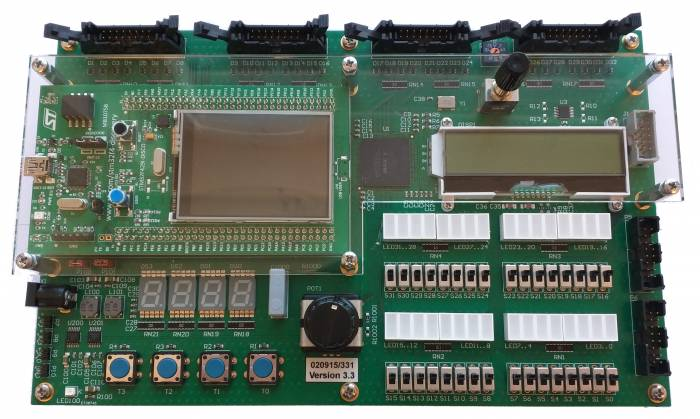
\includegraphics[width=\textwidth]{ctboard}
\caption{Das CT Board, das den Studenten im Modul \glqq Computertechnik 1\grqq{} als Hardware zur Verfügung gestellt wird. (Quelle: ennis.zhaw.ch)}
\label{ctboard}
\end{figure}

Im 21. Jahrhundert noch Hardware an Studierende auszuleihen, mutet schon fast archaisch an. Insbesondere, wenn sich die Hardware leicht als Software simulieren liesse. Und genau hier setzt die vorliegend umgesetzte Idee an: Es soll eine Web-Applikation entwickelt werden, die ein CT Board simuliert und in den \glqq Computertechnik 1\grqq-Praktika an dessen Stelle tritt. Die Studierenden können die Übungen mit dem leichtgewichtigen \glqq Virtual CT Board\grqq{} genauso gut wie mit dem echten Board lösen und brauchen dafür fortan keine Hardware mehr. Die ZHAW kann sich somit die Beschaffung und Wartung von CT Boards sparen.

\subsection{Der Nutzen}

Zwei Zielgruppen werden als Kundschaft anvisiert, nämlich die Informatikstudierenden der ZHAW auf der einen Seite und die ZHAW als Institution auf der anderen Seite. Für beide Gruppen ergeben sich durch das vorliegend entwickelte Produkt unmittelbare Vorteile:

\paragraph{Für die Studierenden:}
\begin{itemize}
\item Die Studierenden des Moduls \glqq Computertechnik 1\grqq{} haben eine elegante Alternative zu den physischen CT Boards und müssen jene nicht mehr nach Hause tragen und für ihre Erhaltung besorgt sein.
\item Im Gegensatz zum bisherigen physischen CT Board benötigt das \glqq Virtual CT Board\grqq{} keinen Strom und lässt sich daher überall - also beispielsweise auch unterwegs - direkt auf dem Laptop starten.
\item Alle Praktika des \glqq Computertechnik 1\grqq-Moduls lassen sich mit dem \glqq Virtual CT Board\grqq{} umsetzen.
\end{itemize}

\paragraph{Für die ZHAW:}
\begin{itemize}
\item Die Lizenz für die vorliegend entwickelte Software ist um einiges preiswerter als die Beschaffung physischer CT Boards. Ausserdemm müssen alte oder defekte Geräte nicht mehr ausgetauscht oder repariert werden.
\item Die Dozierenden müssen für die Praktika nicht mehr mühsam Keil-Projekte konfigurieren. Es genügt, die Assembler-Files ins \glqq Virtual CT Board\grqq{} hochzuladen.
\end{itemize}

\subsection{Abgrenzung zur Konkurrenz}

Es existieren bereits verschiedene Produkte, die den Studenten des Moduls \glqq Computertechnik 1\grqq{} beim Erlernen ihrer Fertigkeiten behilflich sein können.

\paragraph{Virtuelle Emulatoren}
Der Emulator VisUAL von Alman Sarif soll hier stellvertretend für andere virtuelle Emulatoren für die Assembly-Programmiersprache vorgestellt werden. Er wurde ebenfalls für ein Einführungsmodul in die Computerarchitektur entwickelt, allerdings am Imperial College in London. Die Software ermöglicht das Schreiben von Assembly-Code in einem Editor-Fenster, der dann via Button ausgeführt wird und dessen Auswirkungen auf die Register und Flags rechts davon angezeigt werden (siehe Abbildung \ref{emulator}).
\begin{figure}[h]
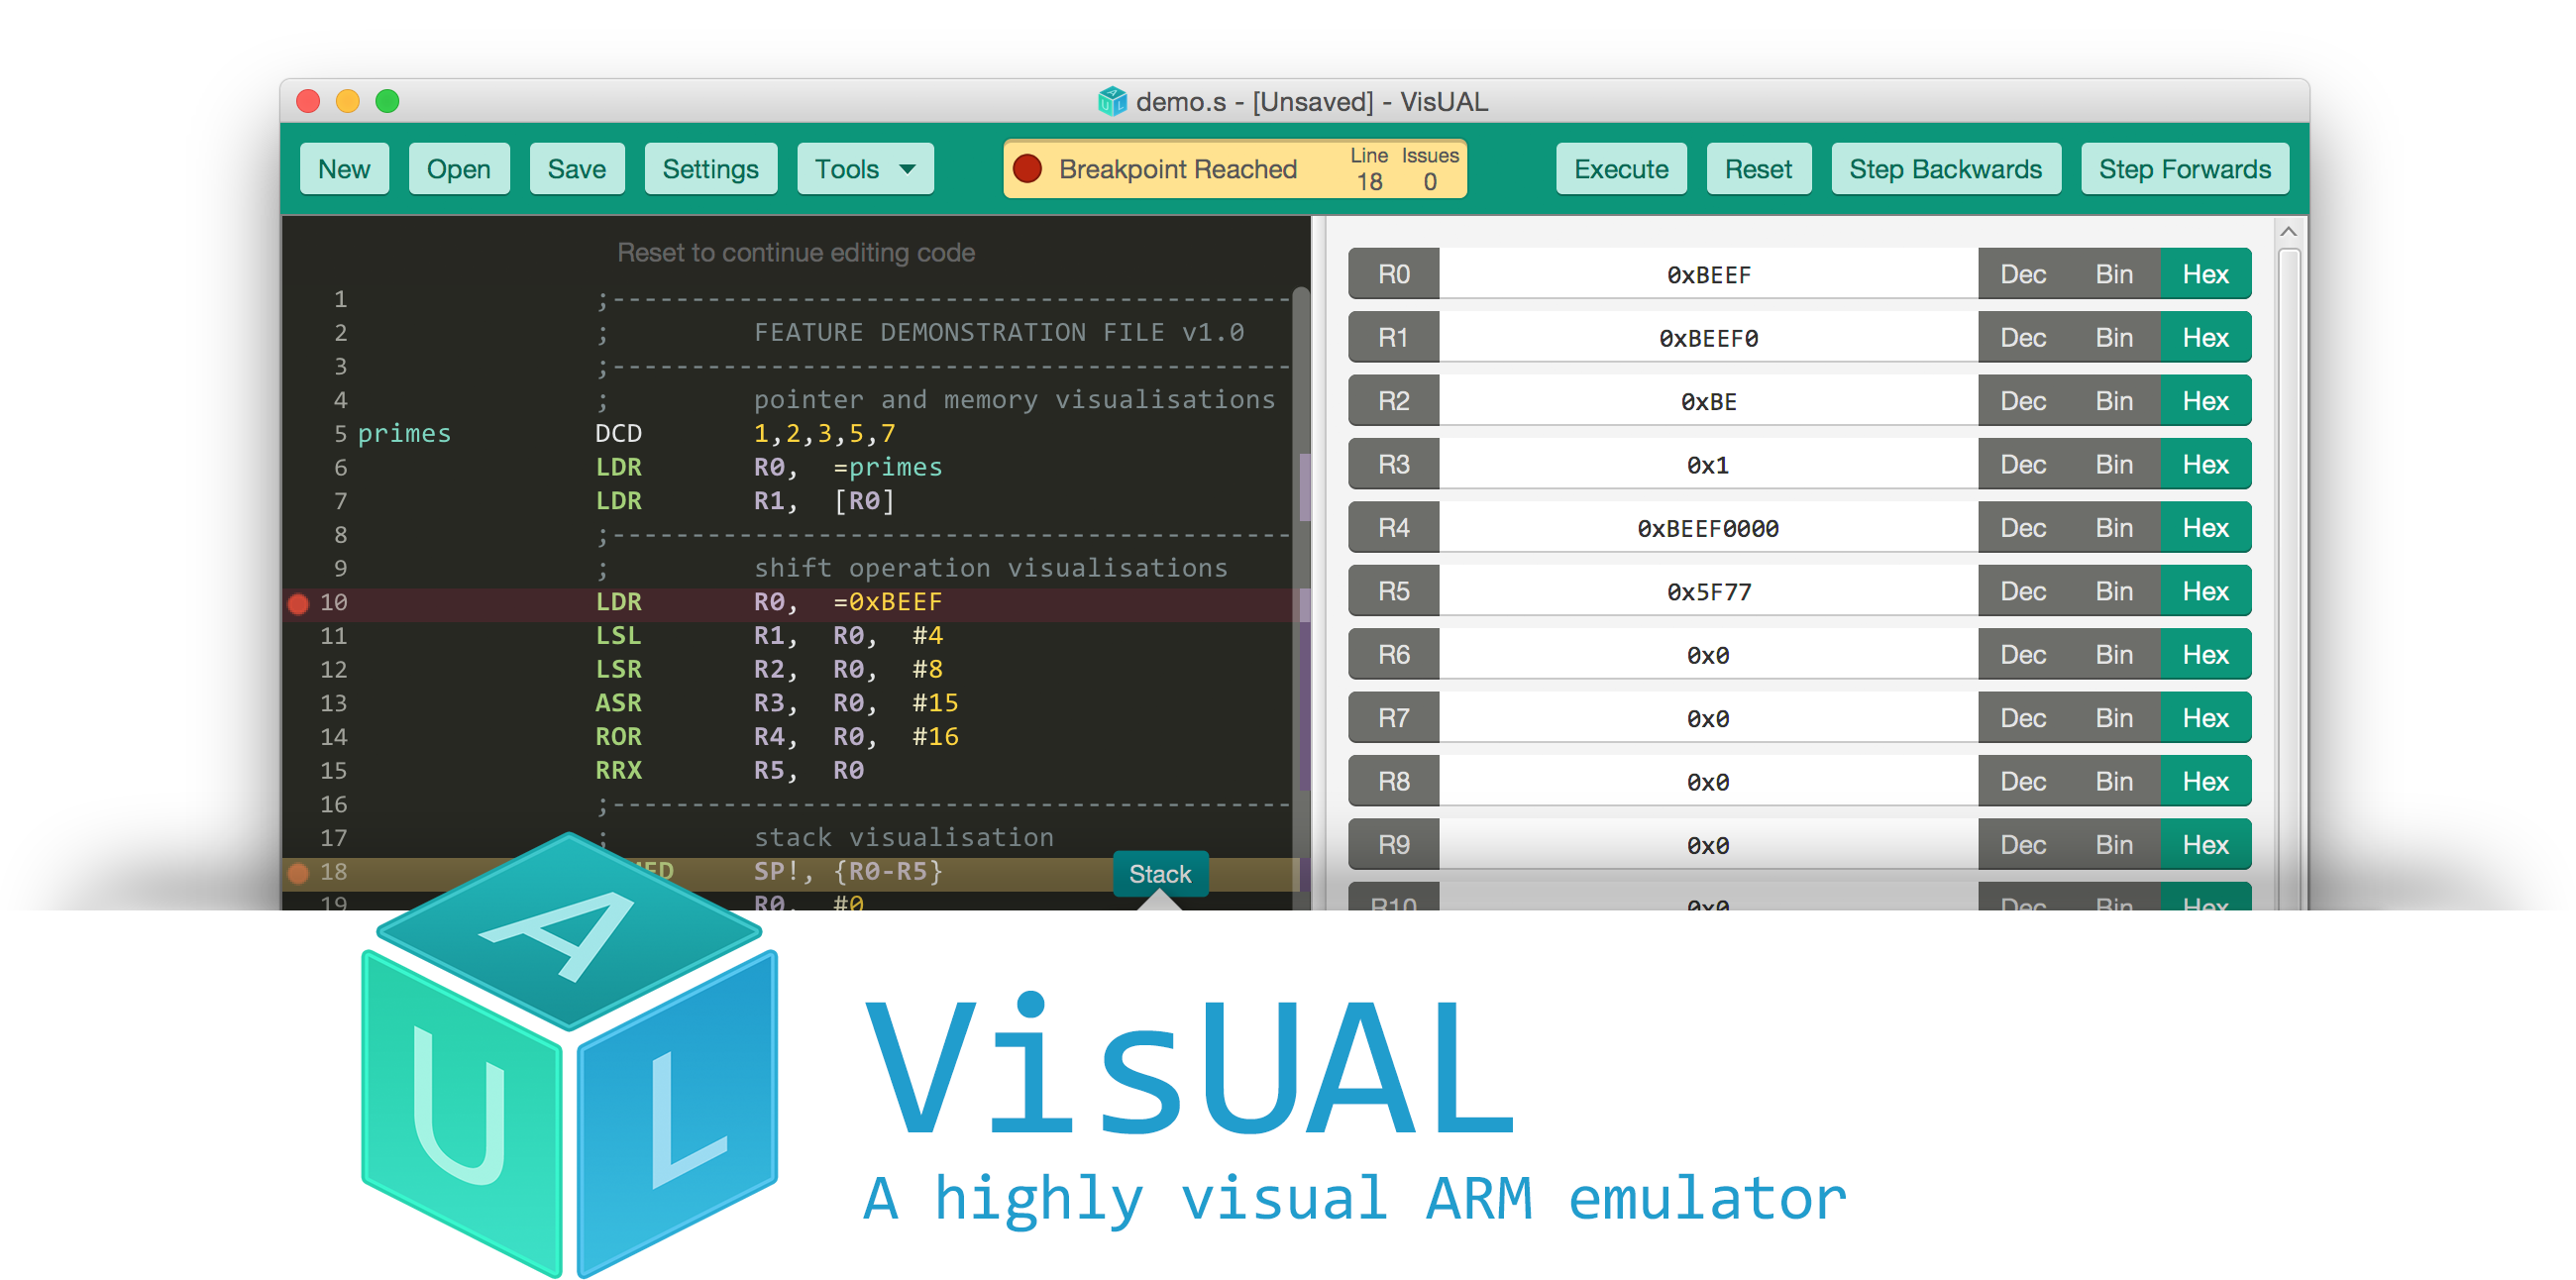
\includegraphics[width=\textwidth]{visual_emulator}
\caption{Der Emulator VisUAL samt seiner grafischen Oberfläche. (Quelle: https://salmanarif.bitbucket.io/visual/index.html)}
\label{emulator}
\end{figure}
Der Unterschied zum \glqq Virtual CT Board\grqq{} besteht darin, dass VisUAL und auch andere Assembler-Emulatoren nicht auf das CT Board ausgerichtet sind, das die \glqq Computertechnik 1\grqq{}-Praktika verlangen. Es gibt bei diesen Programmen keine Visualisierung von Hardware-Bestandteilen, mit Ausnahme der Register und Flags. Das bedeutet, dass diese Emulatoren zwar nützlich sind, um in Assembler zu programmieren, jedoch nicht für die Durchführung der \glqq Computertechnik 1\grqq-Praktika an der ZHAW ausreichen. Das \glqq Virtual CT Board\grqq{} füllt diese Lücke, indem das komplette physische CT Board virtuell visualisiert wird und dieselben Input-/Output-Möglichkeiten bestehen wie beim realen.

\paragraph{Physisches CT Board} 

Das physische CT Board soll hier noch einmal erwähnt werden, da es die Hauptkonkurrenz zum vorliegend entwickelten Produkt darstellt. Es erfüllt die funktionalen Anforderungen der \glqq Computertechnik 1\grqq-Praktika vollumfänglich und ist ausserdem im Schulbetrieb bereits etabliert. Seine Nachteile bestehen insbesondere in seiner Unhandlichkeit. Das \glqq Virtual CT Board\grqq{} soll diesen Nachteil durch seine Virtualität beheben und gleichzeitig dem realen CT Board bzgl. Funktionalität in nichts nachstehen. Damit liegt es im Trend der Zeit, denn Studien belegen, dass die \emph{Digital Natives} der Generation Z den Einsatz aktueller Technologien zur Effizienzsteigerung im beruflichen Umfeld erwarten (West 2018, Wirthman 2020). Somit verhilft das virtuelle CT Board dem Modul \glqq Computertechnik 1\grqq{} bei nachfolgenden Studentengenerationen zu neuer Attraktivität.


\subsection{Risiken}
Trotz ausführlicher und sorgfältiger technischer Analyse des Funktionsumfangs des physischen CT Boards bestehen bei dessen virtuellen Nachbau einige Risiken:
\begin{itemize}
\item Gewisse Funktionen können virtuell nicht gleich nachgebaut werden. 
\item Der Funktionsumfang des virtuellen Boards könnte aufgrund knapper Projektlaufzeit eingeschränkt werden. 
\item Das physische Board besitzt im Verhältnis zum Browsercache ein grosses Memory. Die Software könnte deshalb auf schwächeren Laptops der Studierenden nicht richtig funktionieren. 
\end{itemize}

\section{Resultate}



\section{Diskussion und Ausblick}

\subsection{Weitere Anforderungen}
Die erste Version der Software wird ermöglichen, einen Grossteil der Praktika und Übungen des Moduls \glqq Computertechnik 1\grqq{} virtuell durchzuführen. Sollte die ZHAW eine Weiterentwicklung der Software anstreben, könnten zukünftig auch folgende Funktionalitäten umgesetzt werden: 
\begin{itemize}
\item Implementierung fehlender Funktionen für alle Praktika und Übungen des Moduls \glqq Computertechnik 1\grqq. 
\item Implementierung einer vorbereiteten Bibliothek aller Praktika und Übungen des Moduls \glqq Computertechnik 1\grqq. 
\item Implementierung der Funktionalitäten, welche für das Modul \glqq Computertechnik 2\grqq{} vorausgesetzt sind. 
\item Implementierung einer virtuellen Darstellung von Signalen auf einem Oszilloskop.
\end{itemize}

\subsection{Wirtschaftlichkeit}
Die Einnahmen der nächsten 5 Jahre basieren auf dem Interesse der ZHAW, diese Software weiter zu entwickeln. Zum einen kann bei einem offiziellen Einsatz der Software an der ZHAW eine einmalige Lizenzgebühr von 50'0000 erhoben werden. Diese würde die Kosten der bisherigen Entwicklung decken. Dabei rechnen wir mit einem Preis von 50.- pro Entwicklungsstunde. Hierbei befinden wir uns klar unter dem gängigen Preis auf dem freien Markt. Weitere Funktionalitäten können dabei schrittweise mit einzelnen Upgrades dazugekauft werden. Dabei werden diese Funktionalitäten nur auf Auftrag durchgeführt.

\section{Literaturverzeichnis}

\begin{itemize}

\item[$-$] \emph{https://ennis.zhaw.ch} [abgerufen am 30.03.2022]
\item[$-$] \emph{https://salmanarif.bitbucket.io/visual/index.html}. [abgerufen am 30.03.2022]
\item[$-$] West, Steve (2018). Meeting Millennial Expectations In These Four Areas Of Technology. \emph{https://www.forbes.com/sites/forbestechcouncil/2018/06/28/meeting-millennial-expectations-in-these-four-areas-of-technology/?sh=5df2822f4ffc} [Abgerufen am 25.04.2022]
\item[$-$] Wirthman, Lisa (2020). How Tech-Savvy Millennials Are Driving the Digital Workplace. \emph{https://www.dell.com/en-us/perspectives/how-tech-savvy-millennials-are-driving-the-digital-workplace/} [Abgerufen am 25.04.2022]

\end{itemize}



\end{document}